\documentclass{article}

\usepackage{color,amsmath,amssymb,graphicx,fancyhdr,amsfonts,amsthm,algorithmic,verbatim,bbold,environ}
\usepackage{algorithm,hyperref}
\usepackage{mkolar_definitions}
\usepackage{multirow}
\usepackage[left=2cm,top=2cm,right=2cm]{geometry}
\numberwithin{algorithm}{section}

%%%%%%%%%%%%%%%%%%%%%%%%%%%%%
\newcommand{\tta}{\theta}
\newcommand{\lag}{\left\langle}
\newcommand{\rag}{\right\rangle}
\newcommand{\lnorm}{\left\|}
\newcommand{\rnorm}{\right\|}
%%%%%%%%%%%%%%%%%%%%%%%%%%%%%



\title{CS258 Information Theory Homework 3}
\author{Zhou Litao 518030910407 F1803016}
\date{\today}
\begin{document}
\maketitle

%%%%%%%%%%%%%%%%%%%%%%%%%%%%%%%%%%%%%%%%%%
%%%%%%%%%%%%%                 %%%%%%%%%%%%
%%%%%%%%%%%%%    EXERCISE 1   %%%%%%%%%%%%
%%%%%%%%%%%%%                 %%%%%%%%%%%%
%%%%%%%%%%%%%%%%%%%%%%%%%%%%%%%%%%%%%%%%%%
\begin{exercise}[]{Prove that under the constraint that $X\rightarrow Y \rightarrow Z$ forms a Markov Chain, $X\bot Y | Z$ and $X\bot Z$ imply $X\bot Y$}.
\begin{proof}
  \par{~}
  From $X\bot Y | Z$, we have $I(X;Y|Z)=0$. From $X\bot Z$, we have $I(X;Z)=0$. It follows that 
  \begin{equation}
    \begin{array}{rll}
      I(X;Y) &= H(X) - H(X|Y) &\text{(Unfold by definition of mutual information)}\\[2mm]
      &= H(X) - H(X|Z) + H(X|Z) - H(X|Y) & \\[2mm]
      &= H(X) - H(X|Z) + H(X|Z) - H(X|Y,Z) &\text{(Markov Chain: } p(x|y) = p(x|y,z) \text{)} \\[2mm]
      &= I(X;Z) + I(X;Y|Z) = 0 &\text{(Fold by definition of mutual information)} 
    \end{array}
  \end{equation}
  ,which implies that $X \bot Y$.
\end{proof}
\label{ex1}
\end{exercise}


\begin{figure}[htbp]
  \centering
      \begin{minipage}[t]{0.45\linewidth}
          \centering
          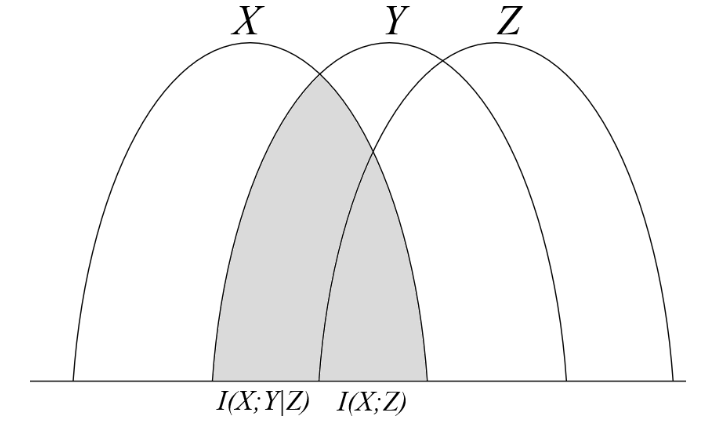
\includegraphics[height=4.5cm]{img/3-1.png}
          \caption{Venn Diagram of Exercise 1}
          \label{fig:ex1}
      \end{minipage}
      \begin{minipage}[t]{0.45\linewidth}
          \centering
          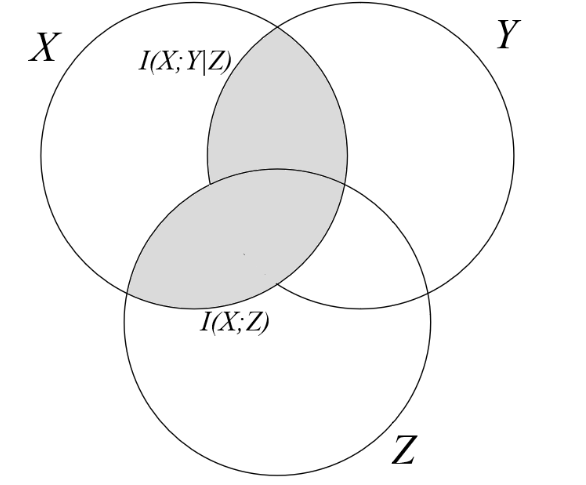
\includegraphics[height=4.5cm]{img/3-2.png}
          \caption{Venn Diagram of Exercise 2}
          \label{fig:ex2}
      \end{minipage}
\end{figure}


%%%%%%%%%%%%%%%%%%%%%%%%%%%%%%%%%%%%%%%%%%
%%%%%%%%%%%%%                 %%%%%%%%%%%%
%%%%%%%%%%%%%    EXERCISE 2   %%%%%%%%%%%%
%%%%%%%%%%%%%                 %%%%%%%%%%%%
%%%%%%%%%%%%%%%%%%%%%%%%%%%%%%%%%%%%%%%%%%
\begin{exercise}[]{Prove that the implication in Exercise \ref{ex1} continues to be valid without the Markov Chain constraint}
  \begin{proof}
    \begin{equation}
      \begin{array}{rll}
        I(X;Y) &= I(X;Y|Z) + (I(X;Y) - I(X;Y|Z)) & \text{(Note } X \bot Y|Z \rightarrow I(X;Y|Z) = 0 \text{)}\\[2mm]
        &= H(X) - H(X|Y) - (H(X|Z) - H(X|Y,Z)) & \text{(Fold by definition of mutual information)}\\[2mm]
        &= (H(X) - H(X|Z)) - (H(X|Y)- H(X|Y,Z)) & \text{(Unfold by definition of mutual information)}\\[2mm]
        &= I(X;Z) - I(X;Z|Y) &  \text{(Note } X \bot Y \rightarrow I(X;Y) = 0 \text{)} \\[2mm]
        &= - I(X;Z|Y) \le 0 & \text{(Nonnegative conditional mutual information)} 
      \end{array}
    \end{equation}
    On the other hand, $I(X;Y) \ge 0$. Hence $I(X;Y)$ must be zero. That is to say, $X \bot Y$.
  \end{proof}
  \end{exercise}

%%%%%%%%%%%%%%%%%%%%%%%%%%%%%%%%%%%%%%%%%%
%%%%%%%%%%%%%                 %%%%%%%%%%%%
%%%%%%%%%%%%%    EXERCISE 3   %%%%%%%%%%%%
%%%%%%%%%%%%%                 %%%%%%%%%%%%
%%%%%%%%%%%%%%%%%%%%%%%%%%%%%%%%%%%%%%%%%%
\begin{exercise}[]{Prove that $Y \bot Z|T$ implies $Y \bot Z|(X,T)$ conditioning on $X \rightarrow Y \rightarrow Z \rightarrow T$.}
  \begin{proof}
    \begin{equation}
      \begin{array}{rll}
        I(Y;Z|X,T) &= H(Y|X,T) - H(Y|Z,X,T) & \text{(Unfold mutual information)} \\[2mm]
        &= H(X,Y,T) - H(X,T) - H(X,Y,Z,T) + H(X,Z,T) & \text{(Unfold conditional entropy)} \\[2mm]
        &= (H(X,Y,T) - H(X,Y,Z,T)) - (H(X,T)-H(T)) &\\[2mm]
        & \quad + (H(X,Z,T)-H(Z,T)) -H(T) +H(Z,T) & \\[2mm]
        &= - H(Z|X,Y,T) - H(X|T) + H(X|Z,T) +H(Z|T) & \text{(Fold conditional entropy)} \\[2mm]
        &= (H(Z|T) - H(Z|Y,T)) - (H(X|T)-H(X|Z,T)) & \text{(Markov Chain: } p(z|x,y,t) = p(z|y,t) \text{)} \\[2mm]
        &= I(Y;Z|T) - I(X;Z|T) & \text{(Note } Y \bot Z|T \rightarrow I(Y;Z|T) = 0 \text{)} \\[2mm]
        &= - I(X;Z|T) \le 0  & \\[2mm]
      \end{array}
    \end{equation}
    On the other hand, $I(Y;Z|X,T) \ge 0$ can be proved by unfolding the definiton of conditional mutual information and the convexity property. Hence $I(Y;Z|X,T)$ must be zero. That is to say, $Y \bot Z|(X,T)$.
  \end{proof}
  \label{ex3}
  \end{exercise}

  \begin{figure}[htbp]
    \centering
        \begin{minipage}[t]{0.45\linewidth}
            \centering
            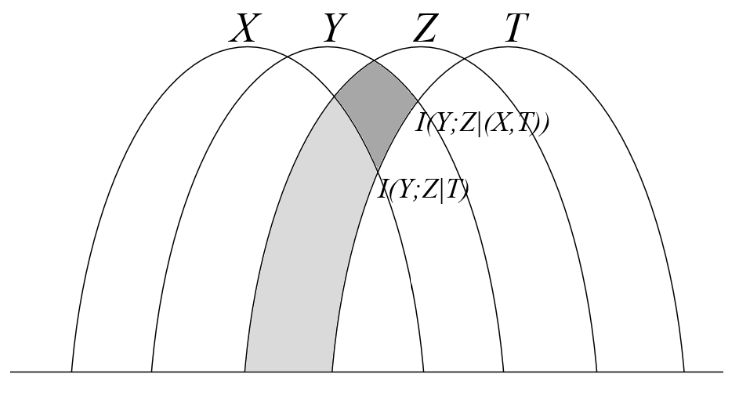
\includegraphics[height=4cm]{img/3-3.png}
            \caption{Venn Diagram of Exercise 3}
            \label{fig:ex3}
        \end{minipage}
        \begin{minipage}[t]{0.45\linewidth}
            \centering
            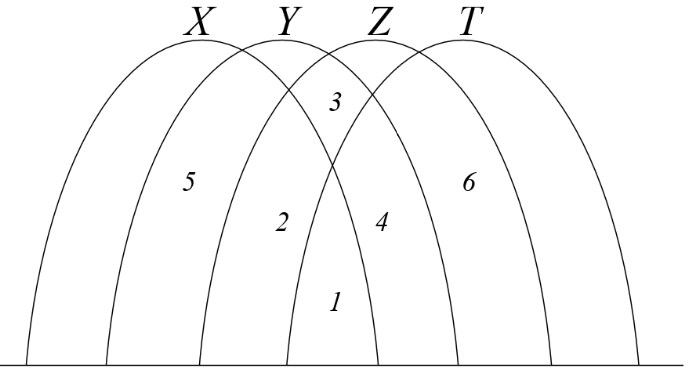
\includegraphics[height=4cm]{img/3-4.png}
            \caption{Venn Diagram of Exercise 4}
            \label{fig:ex4}
        \end{minipage}
  \end{figure}

%%%%%%%%%%%%%%%%%%%%%%%%%%%%%%%%%%%%%%%%%%
%%%%%%%%%%%%%                 %%%%%%%%%%%%
%%%%%%%%%%%%%    EXERCISE 4   %%%%%%%%%%%%
%%%%%%%%%%%%%                 %%%%%%%%%%%%
%%%%%%%%%%%%%%%%%%%%%%%%%%%%%%%%%%%%%%%%%%
\begin{exercise}[]{Let $X \rightarrow Y \rightarrow Z \rightarrow T$ form a Markov Chain. Determine which of the following always hold:
  \begin{enumerate}
    \item $I(X;T)+I(Y;Z) \ge I(X;Z)+I(Y;T)$
    \item $I(X;T)+I(Y;Z) \ge I(X;Y)+I(Z;T)$
    \item $I(X;Y)+I(Z;T) \ge I(X;Z)+I(Y;T)$
  \end{enumerate}
}
  \begin{solution}
    Inequality (1) and (3) always hold. We illustrate the answer through the venn diagram shown in Figure \ref{fig:ex4}, where area 1 $\sim$ 6 is respectively represented by $I(X;T),I(X;Z|T),I(Y;Z|(X,T)),I(Y;T|X),I(X;Y|Z),I(Z;T|Y)$.
    \begin{enumerate}
      \item {
        The inequality can be rewritten in form of areas as
        $$1+(1+2+3+4)\ge (1+2)+(1+4).$$
        Since $I(Y;Z|(X,T))\ge 0$, the inequality holds.
      }
      \item {
        The inequality can be rewritten in form of areas as
        $$1+(1+2+3+4)\ge (1+2+5)+(1+4+6).$$
        We can't determine the relation between $I(Y;Z|(X,T))$ (Area 3) and $I(X;Y|Z)+I(Z;T|Y)$ (Area 5 and 6) except that they are both nonnegative. The inequality will not always hold.
      }
      \item {
        The inequality can be rewritten in form of areas as
        $$(1+2+5)+(1+4+6)\ge (1+2)+(1+4).$$
        Since $I(X;Y|Z)+I(Z;T|Y) \ge 0$ can be proved by the nonnegativity of conditional mutual information, the inequality holds.
        Furthermore, the conclusion can also be derived from the data-processing inequality of Markov Chain with $I(X;Y)\ge I(X;Z)$ and $I(Z;T)\ge I(Y;T)$
      }
    \end{enumerate}
  \end{solution}
\end{exercise}



%%%%%%%%%%%%%%%%%%%%%%%%%%%%%%%%%%%%%%%%%%
%%%%%%%%%%%%%                 %%%%%%%%%%%%
%%%%%%%%%%%%%    EXERCISE 5   %%%%%%%%%%%%
%%%%%%%%%%%%%                 %%%%%%%%%%%%
%%%%%%%%%%%%%%%%%%%%%%%%%%%%%%%%%%%%%%%%%%
\begin{exercise}[Drawing with and without replacement]{An urn contains $r$ red, $w$ white, and $b$ black balls. Which has higher entropy, drawing $k \ge 2$ balls from the urn with replacement or without replacement? Set it up and show why. (There is both a difficult way and a relatively simple way to do this.)}
  \begin{solution}
    We use $X_i \in \left\{ \text{red, white, black} \right\}$ to identify the result of the i-th drawing. No matter with replacement or without replacement, the distributions of a single arbitrary variable $X_i$ are the same.
    \begin{equation}
      \begin{array}{cccc}
        X_i & red & white & black \\
        p(x) & \dfrac{r}{r+w+b} & \dfrac{w}{r+w+b} & \dfrac{b}{r+w+b} \\
      \end{array}
    \end{equation}

    With replacement, the previous result won't interfere with the present drawing. Hence we have $$H\left(X_{i} | X_{i-1}, \ldots, X_{1}\right)=H\left(X_{i}\right)$$. It follows that
    \begin{equation}
      H(X_1,X_2,...,X_k)  = \sum_{i=1}^{k}  H\left(X_{i} | X_{i-1}, \ldots, X_{1}\right) = \sum_{i=1}^{k}H\left(X_{i}\right) \quad \text{with replacement}
      \label{ex5:replace}
    \end{equation}

    Without replacement, we only have
    \begin{equation}
      H(X_1,X_2,...,X_k) = \sum_{i=1}^{k}  H\left(X_{i} | X_{i-1}, \ldots, X_{1}\right) \quad \text{without replacement}
      \label{ex5:noreplace}
    \end{equation}

    Note that in Equation \ref{ex5:replace} and Equation \ref{ex5:noreplace}, all the single-variable entropies are of the same value. By condition-reduce-entropy theorem we know that
    $$H\left(X_{i} | X_{i-1}, \ldots, X_{1}\right) \le H(X_i) \quad \text{for any } i $$

    Since the equality holds if and only if $X_i$ are mutually independent, which is not true in this problem, it follows that the entropy will be larger with replacement.
  \end{solution}
\end{exercise}

%%%%%%%%%%%%%%%%%%%%%%%%%%%%%%%%%%%%%%%%%%
%%%%%%%%%%%%%                 %%%%%%%%%%%%
%%%%%%%%%%%%%    EXERCISE 6   %%%%%%%%%%%%
%%%%%%%%%%%%%                 %%%%%%%%%%%%
%%%%%%%%%%%%%%%%%%%%%%%%%%%%%%%%%%%%%%%%%%
\begin{exercise}[Metric]{A function $\rho(x, y)$ is a metric if for all $x, y$,
  \begin{itemize}
    \setlength{\itemsep}{2pt}
    \setlength{\parsep}{0pt}
    \setlength{\parskip}{0pt}
    \item $\rho (x,y) \ge 0$.
    \item $\rho (x,y) = \rho (y,x)$.
    \item $\rho(x,y)=0$ if and only if $x=y$.
    \item $\rho(x,y)+\rho(y,z)\ge \rho(x,z)$.
  \end{itemize}
  \begin{enumerate}
    \item Show that $\rho(X, Y) = H(X|Y) + H(Y|X)$ satisfies the first, second, and fourth properties above. If we say that $X = Y$ if there is a one-to-one function mapping from X to Y, the third property is also satisfied, and $\rho(X, Y)$ is a metric.
    \item Verify that $\rho(X, Y)$ can also be expressed as
    \begin{equation}\begin{aligned}
      \rho(X, Y) &=H(X)+H(Y)-2 I(X ; Y) \\
      &=H(X, Y)-I(X ; Y) \\
      &=2 H(X, Y)-H(X)-H(Y)
      \end{aligned}\end{equation}
  \end{enumerate}
}
  \begin{proof}
    \par{~}
    \begin{enumerate}
      \item{
        \begin{itemize}
          \item Note that $H(X | Y) \geqslant 0 , \quad H(Y(X) \geqslant 0  \Rightarrow \quad \rho(X, Y) \geqslant 0$
          \item By unfolding the definition it's easy to see \(H(X | Y) \neq H(Y | X)=H(Y | X)+H(X | Y)\)
          \item If $X=Y$, there exists a one-to-one mapping, i.e. \(\rho(X,Y)= H(X | Y)+H(Y|X)=0\)
          
          On the other hand, if \(\rho(X,Y)= H(X | Y)+H(Y|X)=0\)
          Since $H(X | Y) \geqslant 0 , \quad H(Y(X) \geqslant 0$, we have $H(X | Y) = 0 , \quad H(Y(X) = 0$.
          By the conclusion in Exercise 2, Assignment 1, $X$ and $Y$ are mutually each other's function, i.e.there exists a one-to-one mapping between $X$ and $Y$.
          \item The conclusion can be derived using condition-reduce-entropy and nonnegativity of conditional entropy.
            \begin{equation}\begin{aligned}
            H(X | Y)+H(Y | X)+H(Y|Z)+H(Z | Y) & \geqslant H(X| Y,Z)+H(Y | X )+H(Y | Z)+H(Z | Y,X) \\
            &=H(X, Y | Z)+H(Z, Y | X) \\
            &=H(X | Z)+H(Y | X,Z)+H(Z | X)+H(Y | Z,X) \\
            &\geqslant H(X | Z)+H(Z | X)=\rho(X, Z)
            \end{aligned}\end{equation}
        \end{itemize}
        }
        \item {
          \begin{equation}\begin{aligned}
          \rho(X,Y)&=H(X | Y)+H(Y | X)&\\
          &=H(X)-I(X ; Y)+H(Y)-I(X ; Y) &\\
          &=H(X)+H(Y)-2 I(X ; Y) & (\star)\\
          &=(H(X)-I(X ; Y)+H(Y))-I(X ; Y)& \\
          &=H(X,Y)-I(X ; Y) & (\star)\\
          &=H(X,Y)-(H(X)+H(Y)-H(X,Y)) &\\
          &=2 H(X, Y)-H(X)-H(Y) & (\star)
          \end{aligned}\end{equation}
          The expressions required by the problem have been labeled with $(\star)$ in the derivation.
        }
      \end{enumerate}


  \end{proof}
  \end{exercise}

%%%%%%%%%%%%%%%%%%%%%%%%%%%%%%%%%%%%%%%%%%
%%%%%%%%%%%%%                 %%%%%%%%%%%%
%%%%%%%%%%%%%    EXERCISE 7   %%%%%%%%%%%%
%%%%%%%%%%%%%                 %%%%%%%%%%%%
%%%%%%%%%%%%%%%%%%%%%%%%%%%%%%%%%%%%%%%%%%
\begin{exercise}[Entropy of a disjoint mixture]{Let $X_1$ and $X_2$ be discrete random variables drawn according to probability mass functions $p_1(\cdot)$ and $p_2(\cdot)$ over the respective alphabets $X_1 = \left\{ 1, 2, \cdots , m \right\}$ and $X_2 = \left\{m + 1, \cdots , n\right\}$. Let
  \begin{equation}X=\left\{\begin{array}{ll}
    X_{1} & \text { with probability } \alpha \\
    X_{2} & \text { with probability } 1-\alpha
    \end{array}\right.\end{equation}
  \begin{enumerate}
    \item Find $H(X)$ in terms of $H(X_1), H(X_2)$ and $\alpha$.
    \item Maximize over $\alpha$ to show that $2^{H(X)} \le 2^{H(X_1)} + 2^{H(X_2)}$ and interpret using the notion that $2^{H(X)}$ is the effective alphabet
    size.
  \end{enumerate}
  }

  \begin{solution}
    \par{~}
    \begin{enumerate}
      \item {
        We calculate $H(X)$ by unfolding the definition of entropy.
        \begin{equation}
          \begin{aligned}
            H(X) &= - \sum_{x\in X_1} \alpha p_1 (x) \log \alpha p_1 (x) - \sum_{x\in X_2} (1-\alpha) p_2 (x) \log (1-\alpha) p_2 (x) \\
            &= - \alpha \log \alpha \sum_{x\in X_1} p_1 (x) - (1-\alpha) \log (1-\alpha) \sum_{x\in X_2} p_2 (x) + \alpha H(X_1) + (1-\alpha) H(X_2) \\
            &= - \alpha \log \alpha - (1-\alpha) \log (1-\alpha) + \alpha H(X_1) + (1-\alpha) H(X_2)
          \end{aligned}
        \end{equation}
      }
      \item {
        We consider $H(X)$ to be a function over $\alpha$. Note that $g(\alpha)= -\alpha\log(\alpha)$ is a concave function, and some affine transformation over $\alpha$ and linear components won't interfere with the concavity. The function of $H(x)$ is a concave function.

        We can get the maximal value by calculating the derivative of $H(X)$ over $\alpha$.
        \begin{equation}
          \begin{aligned}
            \frac{dH(X)}{d\alpha} &= - \frac{1}{d\alpha} \left(\frac{\alpha \ln \alpha}{\ln 2} + \frac{(1-\alpha)\ln(1-\alpha)}{\ln 2} - \alpha H(X_1) - (1-\alpha) H(X_2) \right) \\
            &= - \frac{1 + \ln \alpha}{\ln 2} - \frac{-1 - \ln(1-\alpha)}{\ln 2} + H(X_1) -H(X_2) := 0 \\
          \end{aligned}
        \end{equation}
        The maximal value is obtained at the derivative to be $0$.
        \begin{equation}
          \begin{aligned}
            -\ln \alpha + \ln (1-\alpha) &= \ln2 \left(H(X_2)-H(X_1)\right) \\
            \ln \frac{1-\alpha}{\alpha} &= \ln2 \left(H(X_2)-H(X_1)\right) \\
            \frac{1-\alpha}{\alpha} &= 2^{H(X_2)-H(X_1)} \\
            \alpha &= \frac{2^{H(X_1)}}{2^{H(X_2)}+2^{H(X_1)}}
          \end{aligned}
          \label{eqn:ex7}
        \end{equation}
        The optimal solution is in the domain, so the maximal value can be obtained. By substituting the $\alpha$ value into $2^{H(X)}$ we can obtain its upper bond.
        \begin{equation}
        \begin{aligned}
          2^{H(X)} &= 2^{- \alpha \log \alpha - (1-\alpha) \log (1-\alpha) + \alpha H(X_1) + (1-\alpha) H(X_2)} \\
          &= \alpha ^{-\alpha} \cdot (1-\alpha)^{\alpha - 1} \cdot \left(2^{H(X_1)}\right)^{\alpha} \cdot \left(2^{H(X_2)}\right)^{1-\alpha} \\
          &\le \left( \frac{2^{H(X_1)}}{2^{H(X_2)}+2^{H(X_1)}}\right) ^{-\alpha} \cdot \left( \frac{2^{H(X_2)}}{2^{H(X_2)}+2^{H(X_1)}}\right)^{\alpha - 1} \cdot \left(2^{H(X_1)}\right)^{\alpha} \cdot \left(2^{H(X_2)}\right)^{1-\alpha} \\
          &= \left(2^{H(X_1)}+2^{H(X_2)}\right) \cdot 2^{-\alpha H(X_1)} \cdot 2^{-(1-\alpha) H(X_2)}  \cdot \left(2^{H(X_1)}\right)^{\alpha} \cdot \left(2^{H(X_2)}\right)^{1-\alpha} \\
          &= 2^{H(X_1)}+2^{H(X_2)}
        \end{aligned}
        \end{equation}

        An interpretation of this conclusion is that $2^{H(X)}$ is the effective alphabet size of $X$, while $2^{H(X_1)}+2^{H(X_2)}$ is the sum sizes of the effective alphabets $X_1,X_2$. The alphabets of $X_1$ and $X_2$ do not overlap, with independent distribution, and they add up exactly to the alphabet of $X$. 

        If our probability of choice between $X_1$ and $X_2$ is in proportion to their effective alphabet size, as the third line in Equation \ref{eqn:ex7} shows, the resulting $X$ will have the effective alphabet size equivalent to the sum of $X_1$ and $X_2$.

        Otherwise, the unbalanced weight of $X_1$ and $X_2$ will reduce the actual effective alphabet size in $X$, since one variable's excessive occurence will reduce the occurence of the other, so that the latter's effective alphabet size will be less than what it really is.
      }
    \end{enumerate}
  \end{solution}
  \end{exercise}


%%%%%%%%%%%%%%%%%%%%%%%%%%%%%%%%%%%%%%%%%%
%%%%%%%%%%%%%                 %%%%%%%%%%%%
%%%%%%%%%%%%%    EXERCISE 8   %%%%%%%%%%%%
%%%%%%%%%%%%%                 %%%%%%%%%%%%
%%%%%%%%%%%%%%%%%%%%%%%%%%%%%%%%%%%%%%%%%%
\begin{exercise}[Entropy of a sum]{Let $X$ and $Y$ be random variables that take on values $x_1, x_2, \cdots , x_r$ and $y_1, \cdots, y_s$, respectively. Let $Z =
  X + Y$.
  \begin{itemize}
    \item Show that $H(Z|X) = H(Y|X)$. Argue that if $X, Y$ are independent, then $H(Y) \le H(Z)$ and $H(X) \le H(Z)$. Thus, the addition of independent random variables adds uncertainty.
    \item Give an example of (necessarily dependent) random variables in which $H(X) > H(Z)$ and $H(Y) > H(Z)$.
    \item Under what conditions does $H(Z) = H(X) + H(Y)$?
  \end{itemize}
}

\begin{solution}
  \par{~}
  \begin{enumerate}
    \item {
      $Z = X + Y$ indicates that any of the two variable can determine the third variable. That is to say, $$H(X|Y,Z)=H(Y|Z,X)=H(Z|X,Y) = 0$$. By observing $I(Y;Z|X)$ we have
      \begin{equation}
        \begin{aligned}
          I(Y;Z|X) &= H(Y|X) - H(Y|X,Z) \\
          &= H(Z|X) - H(Z|X,Y)
        \end{aligned}
      \end{equation}
      ,which implies that $H(Y|X)=H(Z|X)$.

      If $X$ and $Y$ are independent, $H(X,Y)=H(X)+H(Y)$.
      \begin{equation}
        \begin{aligned}
          H(X,Y,Z) &= H(Z|X,Y) + H(X,Y) = H(X)+H(Y)\\
          &= H(X|Y,Z)+H(Y,Z) = H(Z|X)+H(X) \\
          &= H(Y|X,Z)+H(X,Z) = H(Z|Y)+H(Y) \\
        \end{aligned}
        \label{eqn:ex8}
      \end{equation}

      Equation \ref{eqn:ex8} indicates that $H(Z|X)=H(Y)$ and that $H(Z|Y)=H(X)$. By condition-reduce-entropy theorem we have $H(Z) \ge H(Z|X)$ and $H(Z) \ge H(Z|Y)$. It follows that $H(Y) \le H(Z)$ and $H(X) \le H(Z)$.
    }
    \item {
      An exampling distribution of $X$ and $Y$ can be

      \begin{table}[H]
        \begin{center}  
          \begin{tabular}{|c|c|c|c|}
          \hline
          \multicolumn{2}{|c|}{\multirow{2}{*}{Prob}} & \multicolumn{2}{c|}{$x$}      \\ \cline{3-4} 
          \multicolumn{2}{|c|}{}                      & $0$           & $1$           \\ \hline
          \multirow{2}{*}{$y$}         & $0$          & $\frac{1}{2}$ & $0$           \\ \cline{2-4} 
                                      & $-1$         & $0$           & $\frac{1}{2}$ \\ \hline
          \end{tabular}
        \end{center}
      \end{table}

      The entropy of $X$ and $Y$ are 
      $$H(X)=H(Y) = \frac{1}{2}\log 2 + \frac{1}{2}\log 2 = 1$$
      The distribution of $Z=X+Y$ is $\Pr(Z=0) = 1$, which results in the entropy $H(Z) = 0 < H(X) = H(Y)$.    
    }

    \item {
      From $Z = X + Y$ we know $H(Z)=H(Z) - H(Z|X,Y) = I(X,Y;Z)$.

      $I(X,Y;Z) = H(X,Y)-H(X,Y|Z)$ indicates that $H(Z) \le H(X,Y)$. The equality holds if and only if $H(X,Y|Z) = 0$.
      
      Furthermore, $H(X,Y) = H(X) + H(Y) - I(X;Y)$, which implies that $H(X,Y)\le H(X) + H(Y)$. The equality holds if and only if $I(X;Y) = 0$, i.e. $X$ and $Y$ are independent.

      The second equality constraint and the propositions that $H(X|Y,Z)=H(Y|Z,X) = 0$ can ensure the first equality constraint. Therefore, under the condition that $X$ and $Y$ are independent will $H(Z) = H(X) + H(Y)$ hold.
    }
  \end{enumerate}
\end{solution}
\end{exercise}

%%%%%%%%%%%%%%%%%%%%%%%%%%%%%%%%%%%%%%%%%%
%%%%%%%%%%%%%                 %%%%%%%%%%%%
%%%%%%%%%%%%%    EXERCISE 9   %%%%%%%%%%%%
%%%%%%%%%%%%%                 %%%%%%%%%%%%
%%%%%%%%%%%%%%%%%%%%%%%%%%%%%%%%%%%%%%%%%%
\begin{exercise}[Data processing]{Let $X_1 \rightarrow X_2\rightarrow  X_3 \rightarrow \cdots \rightarrow X_n$ form a Markov chain in this order; that is, let
  $$p\left(x_{1}, x_{2}, \ldots, x_{n}\right)=p\left(x_{1}\right) p\left(x_{2} | x_{1}\right) \cdots p\left(x_{n} | x_{n-1}\right)$$

  Reduce $I(X_1;X_2, \cdots , X_n)$ to its simplest form.
  }

  \begin{solution}
    By the chain rule of mutual information we have
    $$I\left(X_{1}; X_{2}, \ldots, X_{n}\right) =\sum_{i=2}^{n} I\left(X_{i} ;  X_1 | X_{i-1}, X_{i-2}, \ldots, X_{2}\right) $$
    Note that for $i>2$, we have
    \begin{equation}
      \begin{aligned}
        I\left(X_{i} ;  X_1 | X_{i-1}, X_{i-2}, \ldots, X_{2}\right) &= H\left(X_i|X_{i-1}, X_{i-2}, \ldots, X_{2}\right ) - H\left(X_i|X_{i-1}, X_{i-2}, \ldots, X_{2}, X_{1}\right ) \\
        &= H(X_i|X_{i-1}) - H(X_i|X_{i-1}) = 0 \quad \text{(Markov Chain)}
      \end{aligned}
    \end{equation}
    It follows that $I\left(X_{1}; X_{2}, \ldots, X_{n}\right) =  I\left(X_{1} ;  X_2 \right) $.


  \end{solution}
\end{exercise}


%%%%%%%%%%%%%%%%%%%%%%%%%%%%%%%%%%%%%%%%%%
%%%%%%%%%%%%%                 %%%%%%%%%%%%
%%%%%%%%%%%%%    EXERCISE 10  %%%%%%%%%%%%
%%%%%%%%%%%%%                 %%%%%%%%%%%%
%%%%%%%%%%%%%%%%%%%%%%%%%%%%%%%%%%%%%%%%%%
\begin{exercise}[Infinite entropy]{This problem shows that the entropy of a discrete random variable can be infinite. Let $A = \sum_{n=2}^{\infty} (n \log^{2} n)^{-1}$. [It is easy to show that $A$ is finite by bounding the infinite sum by the integral of $(x \log^{2} x)^{-1}$. ] Show that the integer-valued random variable $X$ defined by $\text{Pr}(X = n) = (An \log^2 n)^{-1}$ for $n = 2, 3, \cdots,$ has $H(X) = +\infty$.}

  \begin{proof}
    By definition of entropy we can calculate that
    \begin{equation}
      \begin{aligned}
        H(X) &= - \sum_{n = 2}^{\infty} p(n)\log p(n) \\
        &= \sum_{n=2}^{\infty} (An\log^2 n)^{-1} \log (An\log^2 n) \\
        &= \sum_{n=2}^{\infty} \frac{\log A + \log n + \log^2 n}{An\log^2 n} \\
        &= \log A + \sum_{n=2}^{\infty} \frac{1}{An\log n} + \sum_{n=2}^{\infty} \frac{\log^2 n}{An\log^2 n} \\
      \end{aligned}
    \end{equation}
    As has been indicated by the condition, the first component is finite. The last component will be nonnegative with sufficiently large $n$. We show that the second component is infinite. Note that
    $$0 <  \sum_{n=2}^{\infty} \frac{1}{An\log n} < \int_{2}^{\infty} \frac{\ln 2 dx}{A x \ln x} = \int_{2}^{\infty} \frac{\ln 2 d(\ln x)}{A \ln x} = \frac{\ln 2}{A} \ln(\ln x) \bigg|_{2}^{\infty} \rightarrow \infty$$
    It follows that $H(X)=+\infty$
  \end{proof}
\end{exercise}

\end{document}
